% program VLNA -- prida ~ tam kde je potřeba je soucasti texlive baliku
\pdfoutput=1
\documentclass[oneside,12pt]{article}
\usepackage[utf8x]{inputenc}
\usepackage[czech]{babel}
\usepackage{dipp}
\usepackage{listings}
\usepackage{pgfplots, pgfplotstable}
\usepackage{filecontents}
\usepackage{comment}
\usepackage{listings}
\usepackage[export]{adjustbox}
\usepackage{float}

%
%
% START
\begin{document}

\def\,{\penalty10000\hskip.25em}
\pagestyle{headings}
\cislovat{2}
\bakalarska
\titul{Hra založená na rozšířené realitě pro platformu iOS}{Aleš Kocur}{Ing. David Procházka, Ph.D.}{Brno~2014}

\obsah

\newpage
%
% Přehled  literatury
%
\kapitola{Úvod}
% 
% Úvod
Myšlenku rozšířené reality (angl. Augmented reality) nastínil již před více než sto lety americký spisovatel Lyman Frank Baum \cite{baum}, ale až v posledních letech s nástupem mobilních technologií získává na svém potencionálu více než kdy předtím. Mobilní technologie a přenositelná zařízení nám umožňují pomocí senzorů snímat realitu a obohacovat ji o uměle vytvořené prvky. Toho se dá využít v celé škále odvětví jako je zábavní průmysl, medicína, marketing, vzdělávání, navigace, sport a mnoho dalšího. Tato práce se bude zabývat aplikací rozšířené reality v zábavním průmyslu, konkrétně hrami. 

Jednou z populárních her je hra ARhrrrr!, která využívá vytištěné hrací plochy k vizualizaci části města, kterou napadají zombie a hráč v roli snipera v helikoptéře se pohybuje nad hrací plochou a střílí. Tento koncept herní plochy kombinované s interakcí pomocí mobilního zařízení využívá většina her a to z důvodu zachování veškeré uživatelské interakce na jednom místě, na zařízení. Například hra ARDefender požaduje vytištění markerů, na kterých si hráč následně postaví věže které střílí a nebo jiným způsobem interagují. Zároveň uživatel může markery posouvat a tím rozestavovat věže do jiných uskupení.

Vývoj her s rozšířenou realitou je stejně jako vývoj jakýchkoliv her složitý a časově náročný. Proto je důležitá správná volba frameworků zajišťující určité oblasti vývoje jako je v tomto případě vykreslování 3D modelů, animace, rozpoznávání markerů a podobně. Většina dostupných frameworků pro práci s rozšířenou realitou sdružuje všechny zmíněné oblasti do jednoho řešení a navíc nabízí i další funkce nebo multiplatformnost. Mezi nejznámnější frameworky patří ARToolKit, Metaio, Qualcomm Vuforia a Augmented kit. Další cestou jak vytvářet rozšířenou realitu v mobilních aplikacích je pak kombinace několika frameworků pro jednotlivé součásti. Analýzu obrazu dokáže zajistit opensource framework OpenCV, 3D modely a jejich animaci pak také opensource framework Cocos3d nebo komerční Unity, nicméně toto řešení vyžaduje velmi hluboké znalosti matematiky spojené s 3D modelováním pro získání stejného efektu jako při použítí komplexního řešení typu Metaio.


\kapitola{Cíl práce a metodika}
\sekce{Cíl práce}
Cílem práce je prozkoumat možnosti her v rozšířené realitě na mobilní plaformě iOS a vytvořit hru, které bude rozšířené reality využívat jako obohacujícího prvku pro hráče. Prvním a zároveň velmi důležitým krokem je zvolení správného frameworku na základě výše uvedených kritérií. Poté je potřeba důkladně navrhnout herní systém a jak a do jaké míry se bude hra odehrávat v rozšířené realitě. Dalším krokem bude zaopatření grafických podkladů a modelů pro hru a poslední krok spočívá v samotné implementaci.

\sekce{Metodika}
Prvním a zároveň velmi důležitým krokem bude zvolení správného frameworku na základě kriterií, mezi něž patří rychlost vykreslování, licencování a dokumentace. Poté je potřeba důkladně navrhnout herní systém a jak a do jaké míry se bude hra odehrávat v rozšířené realitě. Dalším krokem bude zaopatření grafických podkladů a modelů pro hru a poslední krok spočívá v samotné implementaci.

\kapitola{Rešerše frameworků a konceptů}

\sekce{Frameworky}
Frameworků pro iOS poskytující možnosti práce s rozšířenou realitou existuje velká škála, ale pouze málo z nich je komplexních a dobře zdokumentovaných, aby mohli sloužit k vytvoření hry.

\podsekce{ARToolKit}
ARToolkit byl původně vyvinut Hirokazu Katou na Nara Institute of Science and Technology v roce 1999. Nyní je udržován jako open source projekt s komerčníma licencema od ARToolWork. Tento framework je dostupný pro všechny majoritní platformy (Windows, Linux, Mac OS X, SGI) s různými porty pro mobilní operační systémy (iOS, Android). Mezi jeho hlavní fukce patří kamerově pozicováné a orientováné sledování, sledování černých čtverců s možností definice vlastních typů, jednoduchá kalibrace kamer. Většinou je využit v projektech jako část komplexního toolkitu pro práci s rozšířenou realitou např. OSGART (kombinace ARToolKit a OpenSceneGraph) nebo ARToolKitPlus (rozšířená verze ARToolKitu).

\podsekce{Metaio}
Metaio je multiplatformní framework který vyvíjí stejnojmenná německá firma od roku 2003. Mezi produkty Metaio najdeme framework pro rozšířenou realitu na všechny majoritní platformy a také sadu aplikačních nástrojů specializující se na usnadnění práce i samotný vývoj bez programování. Metaio pro iOS je dostupné jako C++ framework. V dokumentaci k tomuto frameworku lze nalézt příklady základní implementace jednotlivých funkcí.
Dokumentace také uvádí měření, ukazující udržení výkonu vykreslování 60 snímků za vteřinu při 200 000 polygonech na iPhone 5S.

\begin{figure}[H]
    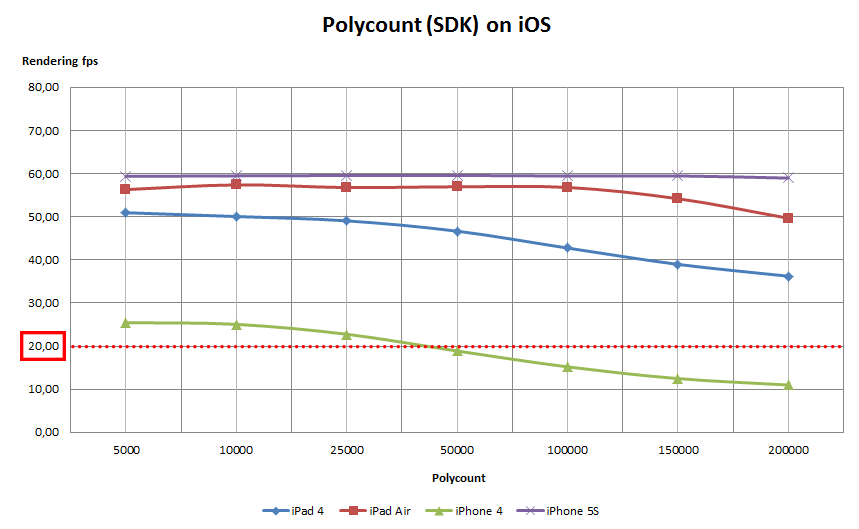
\includegraphics[width=320px, center]{Polycount_SDK_iOS_20fps.png}
    \caption{Metaio polycount}
    \label{fig:awesome_image}
\end{figure}

%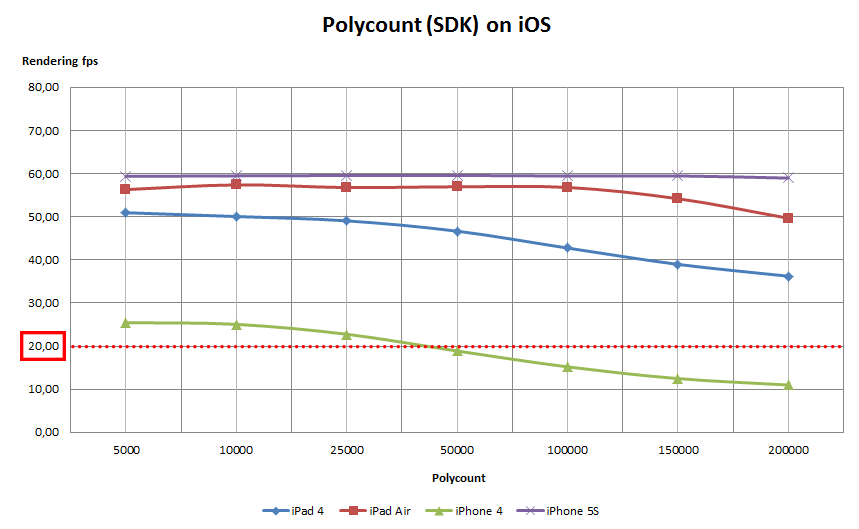
\includegraphics[width=400px]{Polycount_SDK_iOS_20fps}

\podsekce{Qualcomm Vuforia}
Jedná se o poměrně nový framework vyvíjený od roku 2011 a nabízí velké množství funkcí. Jako hlavní lze uvést tzv. markerless recognition (možnost vykreslovat objekty nad obrázky), podporu frameworku Unity (framework usnadňující vývoj 3D her) nebo takzvané virtuální tlačítka (Virtual buttons, tlačítka promítaná do virtuální reality a interakce s nimi). Samotný framework nabízí aplikační rozhraní pro C++, Javu, Objective-C a .NET, což významným způsobem usnadňuje portace aplikace na různé platformy. Široké spektrum funkcí se odráží na licenčních podmínkách frameworku, u neplacených licencí je omezen počet rozpoznaných objektů. 

\podsekce{Augmented kit}
Framework psaný čistě pro platformu iOS a tedy v Objective-C. Vyniká jednoduchým API a dobrou dokumentací. Nabízí pouze základní služby vykreslovaní objektů na markerech, či GPS souřadnic a gyroskopu. Framework je vyvíjen teprve od roku 2012 firmou Luteg Software Technologies a to se projevuje velmi malou vývojářskou základnou. Na druhou stranu má přívětivé licenční podmínky, kdy poskytuje volnou licenci pod podmínkou vodoznaku a nemožnosti aplikaci publikovat na AppStore. 

\sekce{Koncepty}
Koncepty interakce s rozšířenou realitou můžeme rozdělit do třech kategorií.

\podsekce{Interakce se zařízením}
Veškerá interakce hráče probíhá pouze na zařízení, hráč vůbec nemanipuluje s prvky herního pole. Tento koncept je vhodný pro zejména pro typy her ve kterých nepotřebujeme pohybovat s objekty.

\podsekce{Interakce s herní deskou}
Dalším konceptem je interakce s herní deskou, kdy hráč interaguje pomocí gest nebo stisknutím virtuálních tlačítek na desce. Tento koncept štěpí interakční část a zobrazovací (hráč manipuluje s prvky na desce, ale výsledek vidí pouze přes zařízení) a pro uživatele může být v některých případech obzvlášť nepříjemný na ovládání.

\podsekce{Smíšená interakce}
Tento koncept kombinuje předchozí dva uvedené. Hráč v tomto případě primárně používá zařízení, ale má i možnost ovládat herní prvky v reálném prostřední na herní desce. Jako příklad lze uvést výše zmíněnou hru ARhrrrr!, kdy hráč může položit bonbony Skittles na herní plochu a hra je po rozpoznání bere jako miny, které, po střelbě do nich, vybouchnou.

\kapitola{Závěr}
Jako nejvhodnější frameworky se na základě kritérií jeví Vuforia od Qualcommu a Metaio. Oba frameworky vynikají svou rychlostí a srozumitelností aplikačního rozhraní. Metaio nabízí navíc spoustu dolňkových nástrojů pro urychlení práce. Hlavní rozdíl činí licencování, Metaio nabízí studentskou licenci, která je omezena pouze nemožností publikovat aplikaci na App store. Proto jsem pro vývoj hry použil Metaio. 

Při výběru konceptu interakce bylo hlavními kritérii jednoduchost a přímočarost ovládání. Z tohoto důvodu bude hra využívat konceptu \textit{Interakce se zařízením}.

\begin{literatura}

%\citace{apple_library}{APPLE, 2014}
%{
%	\autor{APPLE, INC.}
%	\nazev{iOS developer library}
%	[online]. [cit. 2014-12-18]. Dostupné z: %https://developer.apple.com/library/ios/navigation/	
%}

%\citace{core_data}{APPLE, 2014}{
%	\autor{APPLE, INC.}
%	\nazev{Core Data Programming Guide}
%	[online]. [cit. 2014-12-18]. Dostupné z: https://developer.apple.com/library/ios/documentation/Cocoa/Conceptual/ CoreData/cdProgrammingGuide.html
%}

\citace{baum}{BAUM, 1901} {
	\autor{L. Frank Baum}
	\nazev{The Master Key: An Electrical Fairy Tale, Founded Upon the Mysteries of Electricity and the Optimism of Its Devotees}
	BiblioBazaar, 2006, ISBN 978-1426409240
}

%\citace{neuburg}{NEUBURG, 2013}{
%	\autor{NEUBURG, Matt}
%	\nazev{Programming iOS 6. 3rd edition}
%	Sebastopol: O´Reilly, 2013, xxvii, 1154 s. ISBN 978-1-449-36576-9.
%}
%
%\citace{swift}{APPLE, 2014}{
%	\autor{APPLE, INC.}
%	\nazev{The Swift Programming Language}
%	[online]. [cit. 2014-12-18]. Dostupné z: https://itunes.apple.com/us/book-series/swift-programming-series/id888896989?mt=11
%}
%
%\citace{c++}{STROUSTRUP, 2013}{
%	\autor{STROUSTRUP, Bjarne}
%	\nazev{The C++ Programming Language}
%	 Addison Wesley; 4 edition. 2013, 1368 s. ISBN 978-0321563842.
%}

\citace{bimber}{BIMBER, 2005}{
	\autor{BIMBER, Oliver}
	\nazev{Spatial augmented reality: merging real and virtual worlds}
	 Wellesley: A K Peters, 2005, xiii, 369 s. ISBN 15-688-1230-2
}

\citace{furht}{FURHT, 2011}{
	\autor{FURHT, B.}
	\nazev{Handbook of augmented reality}
	New York, NY: Springer, 2011. 746 s. ISBN 978-1-4614-0063-9.
}

\citace{metaio}{Metaio, 2014}{
	\autor{Metaio, gmbh}
	\nazev{Metaio SDK Documentation}
	[online]. [cit. 2014-12-18]. Dostupné z: http://dev.metaio.com/sdk/documentation/
}

\citace{metaio_polycount}{Metaio, 2015}{
	\autor{Metaio, gmbh}
	\nazev{Metaio SDK Documentation - General guidelines}
	[online]. [cit. 2015-02-16]. Dostupné z: http://dev.metaio.com/sdk/documentation/content-creation/3d-animation/polygon-count/general-guidelines/
}

\end{literatura}

\end{document}
